\section[模型]{模型\\Modeling}

在应用工程中,很少发生给定的物理问题是确切的形式:


\[ x_{k}=F_{k-1}x_{k-1}+\epsilon_{k} \]

\[ b_{k}=A_{k}x_{k}+e_{k} \]

\begin{figure}[h]
	\centering
	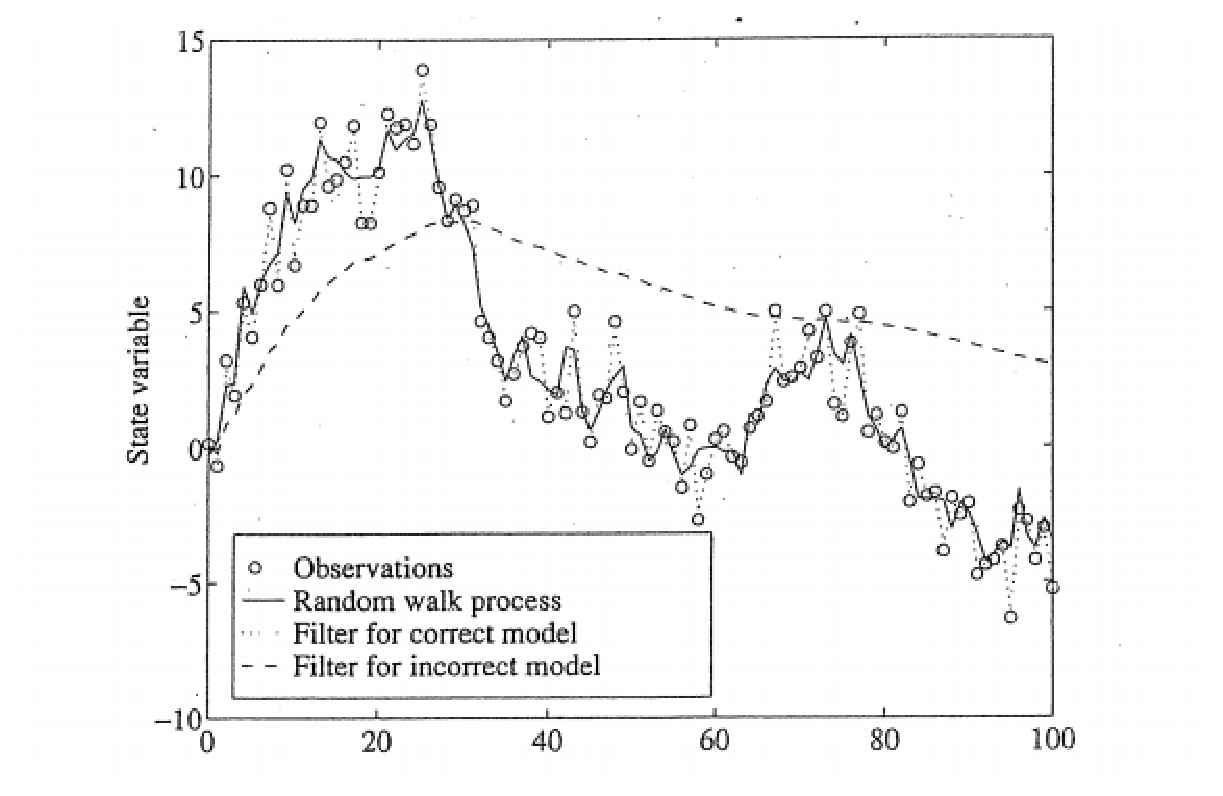
\includegraphics[width=0.7\linewidth]{TeX_files/Part02/chapter05/image/3}
	\caption{Correctly and incorrectly filtered random walk process}
\end{figure}

最常见的是,原始问题必须被修改以适应适当的形式。 这种扭曲通常被称为建模,它在卡尔曼滤波应用中是非常重要的。 良好的建模导致良好的效果; 糟糕的造型导致糟糕的结果。 它是如此简单。 建模过程没有设定规则,它通常需要一些想象力。也许最好变得擅长建模的方法是看各种各样的例子。 我们从Brown and Hwang(1997)的一个例子开始,展示了误差模型的影响。

\textbf{示例5.15}考虑一个实际上是随机游走但是被错误地建模为随机常数 $ c $ 的过程。 然后我们有真正的模型

\[ x_{k}=x_{k-1}+\epsilon_{k}, \quad \epsilon_{k}=单位高斯白噪声,\sigma^{2}{x_{0}}=1 \]

\[ b_{k}=x_{k}+e_{k},\quad k=0,1,2,...\sigma^{2}\left\lbrace e_{k}\right\rbrace =0,1\]

和不正确的模型

\[ x_{k}=c,\quad c~N(0,1) \]
\[ b_{k}=x_{k}+e_{k},\quad k=0,1,2,...\sigma^{2}\left\lbrace e_{k}\right\rbrace=0,1 \]

错误的模型有 $ F_{k}=1,\sum\nolimits_{\varepsilon,k}=0,\sum\nolimits_{e,k}=0.1, \hat{x_{0}}=0 $ 和 $ P_{0}^{-1}=1 $。正确的模型参数是一样的,除了 $ \sum\nolimits_{\varepsilon,k}=1 $,而不是0.

图5.3中显示了100秒的处理结果。还使用另一组N(0,1)个随机数生成该样本处理的测量序列 $ b_{k} $。首先使用不正确的模型处理该测量序列,再次使用正确的模型进行处理。结果与图5.3中的样品过程一起显示。在这种情况下,测量噪声相对较小()$ \sigma\approx 0.3 $,我们注意到,在最初的几个步骤之后,建模过滤器的估计很差。这是由于过滤器的增益随着每个后续步骤而减小。在第100步,增益比起初要低两个数量级。因此,过滤器变得非常缓慢,不会随机游走。如果模拟被允许进一步,那将会变得更加缓慢。


实例5.15就是这样。假设过程或过程的任何方面永远永远永远是永恒的,任何模型都是一个风险模型。在物理世界中,极少数事物绝对不变。这种类型的分歧问题的明显补救办法总是将一些过程噪声插入到每个状态变量中。即使有一定程度的不合适的风险,也可以做到这一点;它造就了比其他方式更安全的过滤器。它也有助于彻底解决潜在的问题。通常,随机游走模型是时间跨度较大的更安全的模型,通常优于超过真正恒定模型的模型。

选择合适的流程模型始终是一个重要的考虑因素。需要一定量的常识判断来决定适合手头情况的模式,但同时不会太复杂。
例如,没有过程会随机游走到无限远。某些地方受到某种限制:对流层短时间内看起来像随机游走。但是假设整天没有测量?我们对对流层方法的了解不足吗?不,当然不。我们知道对流层天顶延迟可以预测为2.4米,约2%的不确定性或更好。

\subsection{计算自相关}

以一个恒定的时间间隔计算一个有序数据集 $ a_{0},a_{1}.1_{2},...a_{n-1} $ 的自相关性是很简单的。 首先我们计算平均值m(平均值)。 第二,我们可以想象数据排列成两行:

\[ shift = 0:\begin{bmatrix}
a_{0}&a_{1}&a_{2}&a_{3}&a_{4}&...\\ a_{0}&a_{1}&a_{2}&a_{3}&a_{4}&...
\end{bmatrix}\quad auto(0)=\sum_{0}^{n-1}a_{i}a_{i}/n \] 


我们将元素  $ a_{i}a_{i} $  相互重叠,并添加。 现在下移一行:

 \[ shift = 1:\begin{bmatrix}
a_{0}&a_{1}&a_{2}&a_{3}&a_{4}&...&\quad\\ \quad&a_{0}&a_{1}&a_{2}&a_{3}&a_{4}&...
\end{bmatrix}\quad auto(0)=\sum_{1}^{n-1}a_{i}a_{i-1}/n \] 

再次,我们将元素相互叠加。 这一次,术语数减少了一个。 我们继续移动,每次我们将总和除以数据数n。 M文件具有以下核心代码:

\[ auto=autocoor(a) \]
\[ m=mean(a) \]
\begin{figure}[h]
	\centering
	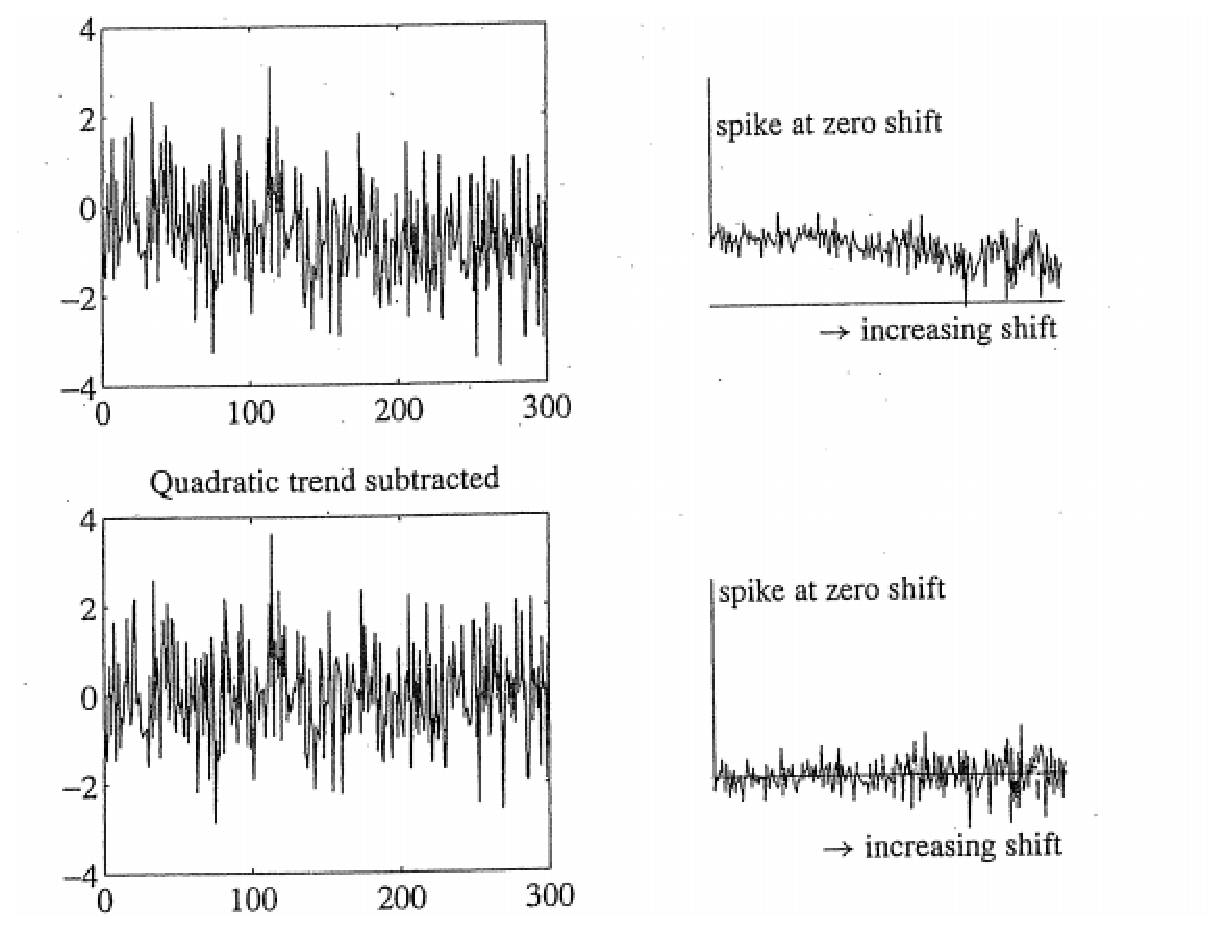
\includegraphics[width=0.7\linewidth]{TeX_files/Part02/chapter05/image/4}
	\caption{Autocorrelation for random data. The peak at zero measures the variance.}
	\label{ }
\end{figure}

 \[ for \quad shift = 0:n-2 \]
\[ q=0 ;\]
\[ for\quad t=1:n-shift \]
\[ q=q+(a(t)-m)*(a(t+shift)-m); \]
\[ end \]
\[ auto(shift+1)=q/n ;\]
\[ end \]


图5.4随机数据的自相关图。 零点的峰值测量方差。

大量转移的总量只包含少量的术语; 重叠数 $ n-shift-1 $ 很小。 统计做法是省略转移产品总额的20%(或类似分数); 他们不那么可靠。 幸运的是,我们对小转换的自相关最感兴趣,因为它们揭示了数据的性质。 所以自动化的结果对于小转换最重要,见图5.4。

我们把总和除以 $  n $,而不是  $ n-shift-1 $ 。这正好确保了

 \begin{equation}\label{5.34}
R=\begin{bmatrix}
auto(0)&auto(1)&...&auto(n-1)\\auto(1)&auto(0)&...&auto(n-2)\\ \colon&\colon&\ddots&\colon\\auto(n-1)&auto(n-2)&...&auto(0)
\end{bmatrix}
\end{equation}

是正半定

\begin{figure}[h]
	\centering
	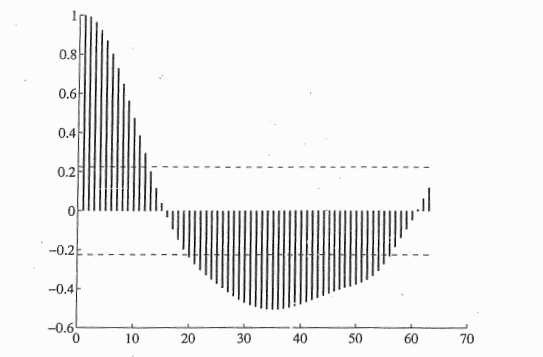
\includegraphics[width=0.7\linewidth]{TeX_files/Part02/chapter05/image/5}
	\caption{Correlogram for an autocovariance function. The dashed horizontal lines represent the limits $ \pm2/\sqrt{n},n $being 80.}
	\label{ }
\end{figure}
图5.5自协方差函数的相关图。 虚线水平线表示极限为$ \pm2/\sqrt{n},n $为80。
\subsection{方差分量模型}

我们再次假设我们的观察(信号)是静止的。 此外,在等距离时间反演中进行了观察。下面将介绍一些分析自相关函数的有用工具。

我们经常会提供标准化的自相关函数。 自相关系数 $ r_{k} $ 定义为

\begin{equation}\label{5.35}
r_{k}=\Re_{x}(k)/\Re_{x}(0),\quad k=0,1,...,n-1 
\end{equation}

变化k的图 $ r_{k} $ 被称为随机过程  $ x_{k} $ 的相关图。 相关图的一个简单的作用是检查观察时间序列中是否存在任何连续依赖性的证据。 为了做到这一点,我们使用一个结果,由于Bartlett表明,对于白噪声序列 $ a_{k} $,对于大的 $ n $,$ r_{k}  $大致正态分布,平均值为零,方差为 $  1 / n $。 因此,
大于 $ 2/\sqrt{n} $ 绝对值的  $ r_{k} $ 值可以在约5%的水平被认为是重要的。 如果计算大量数据  $ r_{k} $ ,即使ajc是白噪声序列,也有可能某些数值超过该阈值。

图5.5显示了接收机时钟偏移的相关图。 从0到12的偏移量超过极限值 $ ± 2/\sqrt{n} $,从$  k = 20 $ 到 $ k = 56 $。相关图表明观测值之间的相关性,即使是高达56个单位时间的变化。

在实践中,随机过程通常显示非随机趋势。 随着噪声 $ \epsilon_{t} $ 我们有

\[ Z_{t}=\mu_{t}+\epsilon{t} \]

我们将通过将第i个系列的观测值 $ Z_{i}(t) $ 分为起始水平  $ L_{i}(t) $ ,随机静止部分 $ M_{i}(t) $ 和噪声 $ N_{i}(t) $ 来演示如何处理这种情况:

\begin{equation}\label{5.36}
Z_{t}(t_{k})=L_{i}(t_{0})+M_{i}(t_{k})+N_{i}(t_{k})
\end{equation}

所有实验对象 $  i = 1,2,...,m $ 的所有观察值在等距离时间  $ t_{0},t_{1},...t_{k},L_{i} $ 被取代,随机变量取决于时间  $ t_{k} $ 时  $ L_{i} $ 在时间 $ t_{0} $  被定义。 $ i\neq j $时  $ L_{i} $独立于 $ L_{j} $,分布为  $ N(0,\lambda^{2}) $ 。 噪音分布为 $ N(0,\nu^{2}) $ ,在时间和主体之间独立。 最终 $ M_{i}(t_{k}) $ 分布为 $ N(0,\mu^{2}) $ ,当$ R(k)=\mu^{2}r(k) $ 和主体之间独立。 我们记得$ r(0) = 1 $和 $ r(k)\rightarrow 0 $时,$ k\rightarrow \infty $。 三个分量 $  L_{i},M_{i}, $和$ N_{i} $ 假定相互独立。观测方差为

\[ R_{Z}(0)=Var(Z_{i}=\lambda^{2}+\mu^{2}+\nu^{2}) \]

$ Z_{i}(t_{l}) $ 和  $ Z_{j}(t_{m}) $ 之间的协方差为


\begin{equation*}
\begin{aligned}
\sigma (Z_{i}(t_{i}), Z_{j}(t_{m}))&=E\left\lbrace Z_{i}(t_{i}) Z_{j}(t_{m})\right\rbrace\\
&=E\left\lbrace(L_{i}(t_{0})+M_{i}(t_{l})+N_{i}(t_{l}))(L_{j}(t_{0})+M_{j}(t_{m})+N_{j}(t_{m}))  \right\rbrace\\
&= E\left\lbrace L_{i}L_{j}\right\rbrace +E\left\lbrace M_{i}(t_{l})M_{j}(t_{m}) \right\rbrace =(Var(L_{i})+\mu^{2}r_{Z}(t_{m}-t_{l}))\delta_{ij}
\end{aligned}
\end{equation*}

注意,由于受试者的独立性,特别是 $ i\neq j $ 时协方差为零。

有一段时间我们对自相关 $ R_{Z}{k} $ 进行了研究。观测误差 $ N_{i}(t_{k}) $ 不等于零; 这意味着  $ k\rightarrow 0 $ 时 $ R_{Z}(k) $ 不接近 $ R_{Z}(0) $ ,$ k\rightarrow \infty $时$ R_{Z}(k) $ 也不接近0。 这是由主题特定的随机变量引起的。


从(5.34)我们记得R,并且E表示一个对角线元素都是1的矩阵,则协方差矩阵可以写为

 \[ \sum = \lambda^{2}E+\mu^{2}R+\nu^{2}I \]
 
 现在我们准备介绍变异函数了
 
 
 \begin{equation}\label{5.37}
V(k) = 1/2E\left\lbrace (Z_{i}(t_{l})-Z_{i}(t_{m}))^{2} \right\rbrace
\end{equation}

 
 我们有
 
  \[ Z_{i}(t_{l})-Z_{i}(t_{m})=M_{i}(t_{l})-M_{i}(t_{m})+N_{i}(t_{i})-N_{i}(t_{m})\]
  
  并记住, $ M_{i} $ 和 $ N_{i} $是独立的。
  
 \begin{equation*}
 \begin{aligned}
 V(k)&=1/2E\left\lbrace (M_{i}(t_{l})-M_{i}(t_{m}))^{2}\right\rbrace+1/2E\left\lbrace (N_{i}(t_{l})-N_{i}(t_{m}))^{2}\right\rbrace\\
 &=\mu^{2}(1-r_{Z}(k))+\nu^{2} 
 \end{aligned}
 \end{equation*}
  

图5.6显示了具有三个方差分量$ \lambda^{2},u^{2} $ 和 $ \mu^{2} $.的变异函数。 记住 $ r_{Z}(0)=1 $,因此 $ lim_{k\rightarrow 0}V(k)=\nu^{2} $。我们可以从图中读取 $ \nu^{2} $ 作为纵坐标轴的截距。

对于我们所用的任何静态,随机过程, $ k\rightarrow 0 $ 时我们有$ r_{Z}(k)\rightarrow 0 $ 。 因此$ V(\infty)=\mu^{2}+\nu^{2} $ 。 因此,个别受试者的差异  $\mu^{2} $ 被发现是$ V(\infty) $ 减去 $ \mu^{2} $。
\begin{figure}[h]
	\centering
	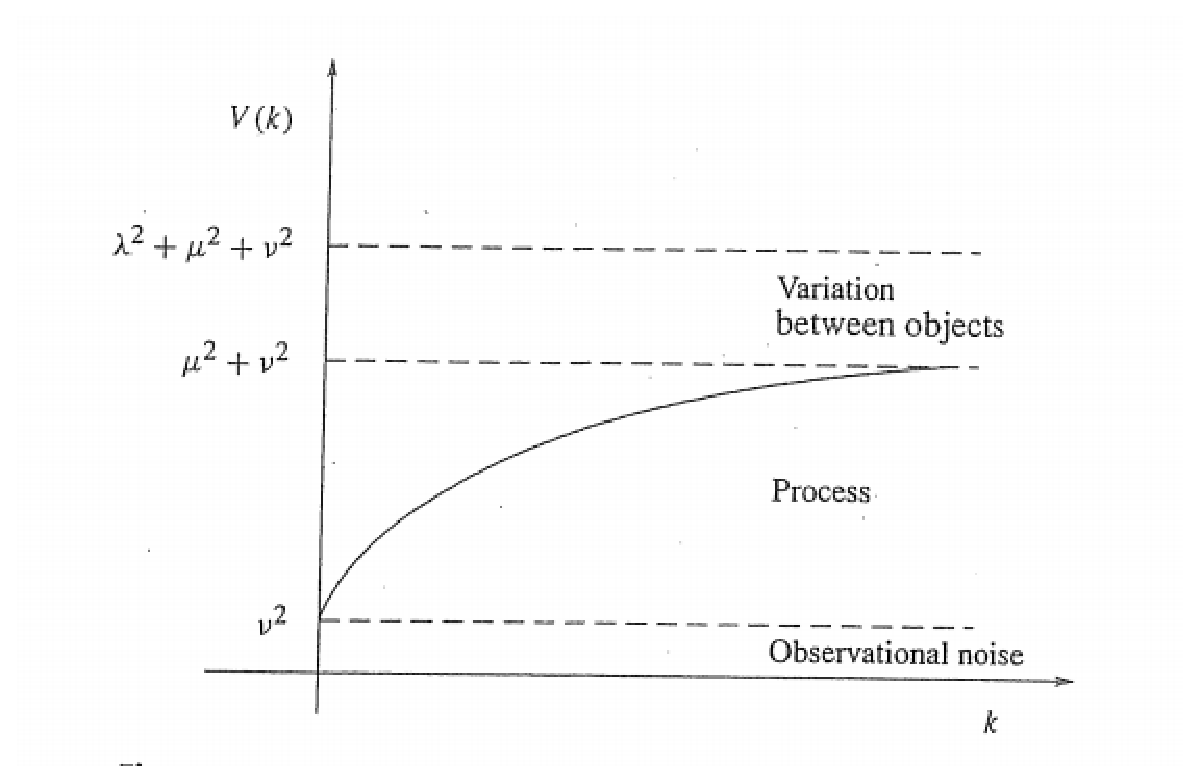
\includegraphics[width=0.7\linewidth]{TeX_files/Part02/chapter05/image/10}
	\caption{Variogram illustrating the three variance components}
	\label{ }
\end{figure}

通过实验对象的数据估计所有观测值$ Z_{i} $的总方差,再次假设过程相互独立,当 $ i\neq j $时,对所有的 $ l ,m,i和j$,总方差被计算为$ (Z_{i}(t_{l})-Z_{j}(t_{m}))^{2}/2 $的均值。这使得  $ M=\sum\nolimits_{i}(_{2}^{n_{i}}) $,其中,$ n_{i} $ 是 $ i $ 序列的观测次数:

 \[ \lambda^{2}+\mu^{2}+\nu^{2}=1/2M \sum_{i\neq j}(Z_{i}(t_{l})-Z_{j}(t_{m}))^{2} \]
 
 总方差如图6所示,人口的方差 $ \lambda^{2} $ 也可以在纵坐标轴中读取。
 
 自相关函数的两个常见例子是指数相关函数
 
\begin{equation}\label{5.38}
r(k)=e^{-\alpha k}
\end{equation}

 和高斯相关函数
 
\begin{equation}\label{5.39}
r(k)=e^{-\alpha k^{2}}
\end{equation}

 
 在图5.7中,我们绘制了(5.38)和(5.39)的自相关函数以及相应的变差函数。 对于小的时间差k,指数相关函数的相关性迅速降低,而高斯相关函数在较大时间内具有强相关性,后迅速下降。
 
 示例5.16为了演示该理论,我们使用接收机和卫星之间作单差。 我们使用具有伪随机噪声码(PRN)2,9,16,23,26和27号卫星。我们集中研究历元k的电离层延迟。我们使用双频观测值以消除延迟$ I_ {k} $中的主要误差:
 
  
 \[ I_{k} =\frac{(\Phi_{2,k}-\lambda_{2}N_{2})-(\Phi_{1,k}-\lambda_{1}N_{1})}{1-(f_{1}/f_{2})^{2}} \]
 
 
\begin{figure}[h]
	\centering
	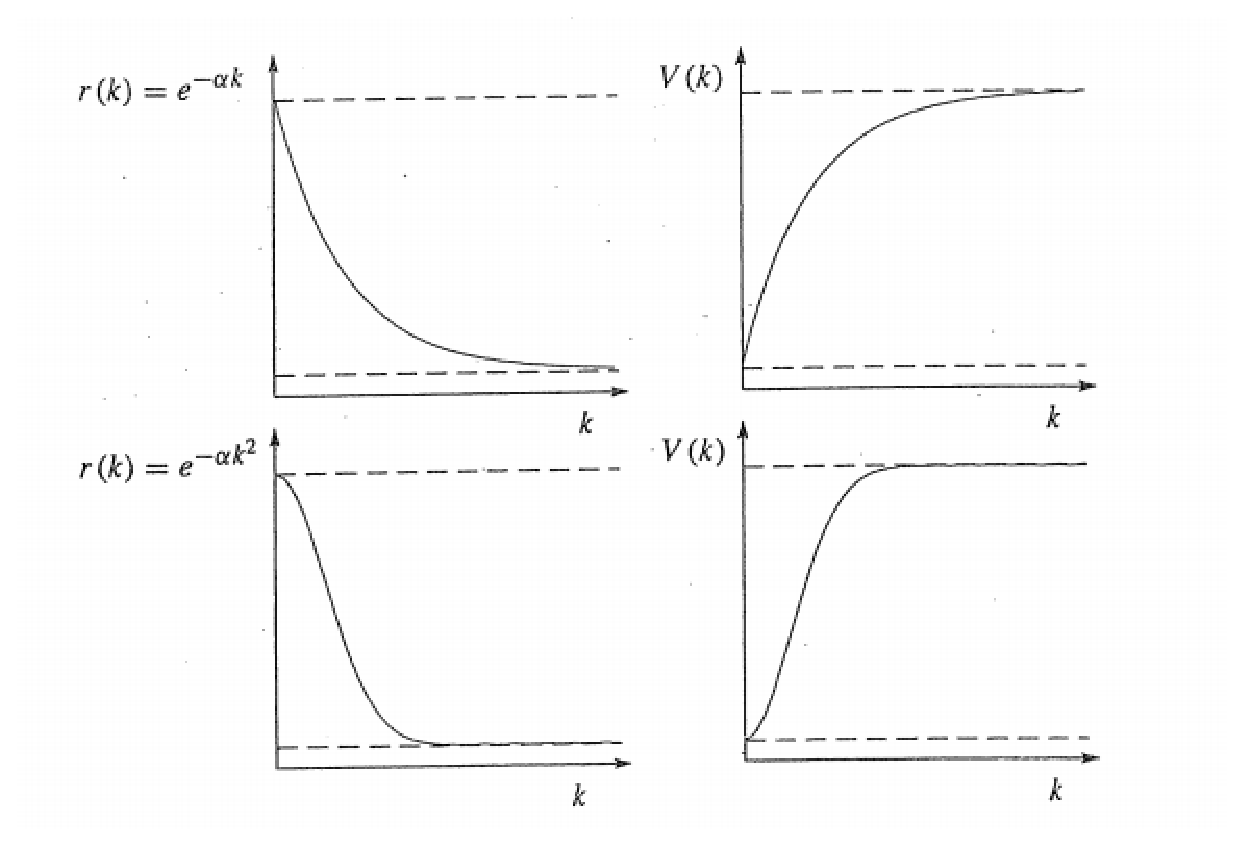
\includegraphics[width=0.7\linewidth]{TeX_files/Part02/chapter05/image/6}
	\caption{Exponential and Gaussian autocorrelationfunctions and variograms}
	\label{ }
\end{figure}

 
 图5.8描述了对于单差的$ I_ {k} $,单差再作差又是所谓的双差。实际基线长度为4.6公里。 对于单差 $ I_ {k} $ 通常在 $ 5-15 $ 米之间变化。 单差的 $ I_ {k} $ 值为2.5-3m,双差为 $ -0.2-0.2 $ 米。 请注意,单个PRN的仰角平均值列于表5.3。 我们可以看到到 $ I_ {k} $ 强烈地依赖于单个卫星的高度角。
 
 现在我们来看 $ I_ {k} $ 的自相关函数。为了消除观测序列中的可能趋势,经常会从历元差 $ I_ {K} -I_ {K-1} $ 开始调查 。图5.9(左上图)显示了2号卫星单差电离层延迟的自相关性。0处的峰值等于单差 $ I_ {K} -I_ {K-1} $ 的方差。现在我们计算非差的自相关性,结果
 
 \[\textbf{ Table 5.3} Autocorrelation of ionospheredelay for one-ways \] 
 \[ \begin{tabular}{lccc}
 \hline
 $ \quad$ & $ Elevation  $ & $\sigma_{1}(m)$&$Shift for firstzero  $ \\
 \cline{1-4}
 $ PRN$ & $ (^{\circ}) $ & $ master \quad rover $&$master \quad rover  $ \\
 $ 26$ & $ 68.9 $ & $ 0.08 \quad0.11 $&$35\quad 30  $ \\
 $ 2$ & $ 59.0 $ & $ 0.08 \quad0.04 $&$15\quad 35  $ \\
 $ 27$ & $ 28.0 $ & $ 0.39 \quad0.35 $&$30\quad 32  $ \\
 $ 16$ & $ 22.8 $ & $ 0.77 \quad0.71 $&$30\quad 30  $ \\
 $ 23$ & $ 20.4 $ & $ 0.17 \quad0.19 $&$12\quad 20  $ \\
 $ 9$ & $ 18.5 $ & $ 0.48 \quad0.19 $&$15\quad 30  $ \\
 
 \hline
 \end{tabular} \] 
 
 
 \begin{figure}[h]
 	\centering
 	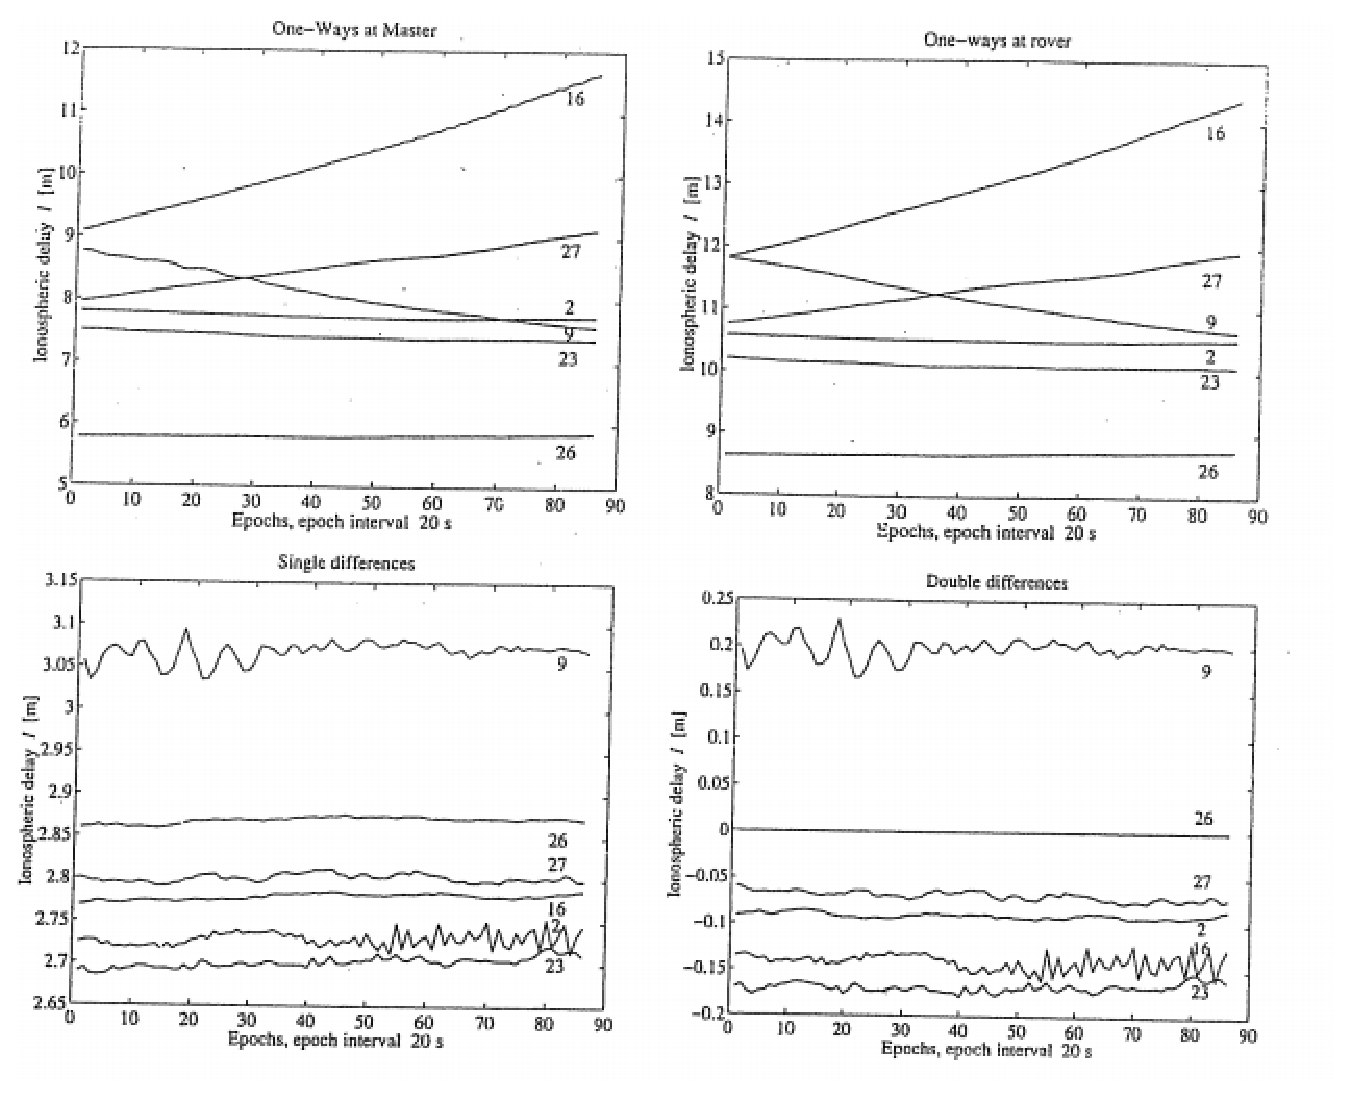
\includegraphics[width=0.7\linewidth]{TeX_files/Part02/chapter05/image/7}
 	\caption{Exponential and Gaussian autocorrelationfunctions and variograms}
 	\label{}
 \end{figure}
 
 如图右上方所示。这显然反应了延迟的系统性。我们的最终目标是对这部分进行建模,然后从实际延迟中减去,希望只留下白噪声或近似白噪声。有一个好的模型,我们可以提高电离层时间延迟 $ \ delta_ {t} $ 以及伪距 $ d $ 估计的精度。
 
 我们继续计算单差中  $ I_{k} $  的自相关值,计算单差的自相关值时必须遵守(5.13)给出的规则,这意味着我们必须计算互相关,图的左下角显示了2号卫星的结果。
 
 从表格5.3中我们得到2号卫星 $ \sigma_{1}=2 $厘米,16号卫星$ \sigma_{1}=77 $厘米,表5.3中的结果是通过调用下列函数产生的:
  \[ one_way(m)(27)\quad and \quad autocorr(x(2,:)^{'}) \]
  
  然而单差的结果减小到4毫米到9毫米,双差的结果减小到2毫米到9毫米,这个例子常用的M文件被称为$ oneway_{i} $。
  
  由于几何变化, $ I_{k} $ 会随着基线长度 $  d = 5, 25, 50, 100,500, 1000 $ 千米而变化,因此,我们建议有兴趣的读者进行探索和调查,最终确定差分电离层的方差 $ \sigma_{0}^{2} $ ,相关时间 $  T  $ ,相关长度 $ D $的关系。
  
  \begin{figure}[h]
  	\centering
  	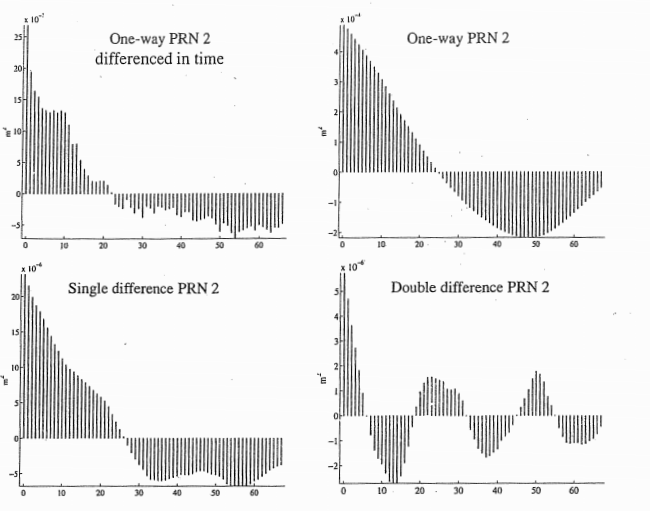
\includegraphics[width=0.7\linewidth]{TeX_files/Part02/chapter05/image/8}
  	\caption{Autocorrelation fo rionospheric delay to PRN 2}
  	\label{ }
  \end{figure}
   图的左上角显示了历元差分的结果,右上角显示了单历元的结果,左下角显示了单差的结果,右下角显示了双差的结果。注意各种数量级,采样间隔 $ \delta_{t} $ 和基线长度 $ d $ 关系如下:
   
   \begin{equation}\label{5.40}
   R_{x}(k,d)=\sigma_{0}^{2}e^{-|\delta_{t}|/T} e^{-d/D}
   \end{equation}
    
    这个函数 $ R_{x} $ 1994年由Goad和Yang通过载波的双差观测值提出。作者假设了一个平稳的指数相关过程:估计 $ T $ 到64分钟, $ \sigma_{0}^{2}=2m^{2} $, D $ \approx $ 1500千米,通常可以调整参数$ \sigma^{2} $和$ \alpha $来调整高斯——马尔科夫过程,在$ k = 0 $时调整$ \sigma_{0}^{2} $, 1/e时调整$ \alpha $。
    
    已知电离层延迟具有明显的日变化。 在Klobuchar(1996)中,我们发现以米为单位的 $ I $ 的近似表达式,作为当地时间 $ t $ 的函数 (以小时计):
    
    \[ I=2.1+0.75\cos((t-14)2\pi/28) \]
    
    该值在天顶方向有效。 为了获得$ I $的增加值,在高度角为1/2个周期的方向($ El $的范围为0-0.5,半个周期时间为$ \ pi $等于弧度),我们必须乘以倾斜因子。
    
     \[ F(El)=1+16(0.53-El)^{3} \]
     
     \begin{figure}[h]
     	\centering
     	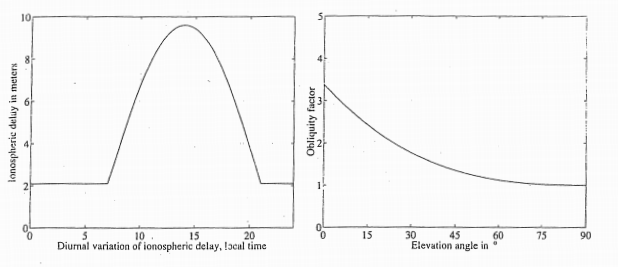
\includegraphics[width=0.7\linewidth]{TeX_files/Part02/chapter05/image/9}
     	\caption{Ionospheric delay model as function of local time and elevation angle}
     	\label{ }
     \end{figure}
     
     该表达式基于IS-GPS-200(2007)中给出的公式。 图5.10显示了$ I $和$ F(El)$的图表。小于2.1m的恒定的延迟表示夜间的延迟。 随着太阳升起,电离层延迟在白天呈现余弦形状。
     
     解释自相关函数时,请记住以下重要属性:
     
     最大值自相关函数的最大值为零移位:
     
      \[ E\left\lbrace x^{2}(t)\right\rbrace  = R_{x}(k) \]
      
      对称条件,自相关函数是一个偶数函数:
      
       \[ R_{x}(k) = R_{x}(-k) \]
       
       而互相关函数满足:
       
        \[ R_{xy}(k)=R_{yx}(-k) \]
        
        均方值互相关由下式决定:
        
         \[ |R_{xy}(k)|^{2}\leq R_{x}(0)R_{y}(0)\leq\frac{1}{2}((R_{x}(0))^{2}+(R_{y}(0))^{2}) \]
         
        周期性,如果 $ x $ 有周期性,则自相关函数也具有周期性。
        
       \textbf{ 备注5.1}(滤波差分技术的理论解释)我们可能会看到由两个单差测量数据 $ S_{i} $: $ D=S_{1}-S_{2} $组成的双差数据$ D $。每个单差测量数据都是简单的由 $ S_{i}=\rho_{i}+t $ 组成,其中 $ \rho_{i} $是伪距,$ t $是接收器时钟偏移乘以$ c $转换得到的长度。
       
       我们说明差分的几个基本事实。一开始有两个单差:
       
        \[ S_{1}=\rho_{1}+t \]
       \[ S_{2}=\rho_{2}+t \]
       
       和他们组成的双差
       
       \[ S_{2}-S_{1}=\rho_{2}-\rho_{1} \]
       
       对双差来说情况有所不同,双差不能估计$ t $,你可以从单差开始估计,但是先验钟差的方差  $ \sigma_{clock}^{2} $ 必须是无穷大,否则的话需要引入第三个观测量,但双差模型中没有。所以一个模型中要有$ S_{1} $, $ S_{2} $和 $ \sigma_{clock}^{2} $,这等价于$ S_{1} $, $ D $和  $ \sigma_{clock}^{2} $。 如果$ \sigma_{clock}^{2} = \infty $,这意味着它没有价值。所以等价于 $ S_{1} $ 和 $ D $。现在,双差不明确涉及钟差,$ S_ {1} $的唯一用途是估计钟差。由于双差不需要估计钟差,所以$ D $ 用来定位。
       
       然而,如果$ \ sigma_ {clock} ^ {2} <\ infty $,那么这将使这三个量结合在一起,在这种情况下,所有这三个测量都将一起处理。使用$S_{1},S_{2},t  $或$ S_{1},D,t $或 $ S_{2},D,t $都无关紧要。如果将时钟视为在每个历元都不同,然后绘制其估计值,您将看到时钟不会随无穷大的方差而漂移。 从理论上说,我们知道有关时钟漂移的一些事情是正确的,使用双差我们无法利用这些知识(因为t消除了)。
       
       现在无法回答的问题是“接收机时钟在什么程度上随机漂移?”明显不同的接收机具有非常大的差异(通常为石英)时钟。 国际地球动力学GPS服务(IGS)提出最好的办法是是用铷或甚至更好的铯振荡器驱动用于轨道计算的接收器。 甚至更好的是氢气,但现在他们太贵了,不予考虑。 那么具有较小方差的更具描述性的随机模型可以证明是有用的。 石英钟相对于厘米的定位要求漂浮得如此之大,试图对它们进行建模对改进位置几乎没有什么影响。所以我们可以得出结论:
       
       - 双重差异可以被认为是过滤器,其中钟差被建模为具有无限方差的白噪声。
       
       - 如果预测的方差小于无穷大,则使用单差分析预测接收机钟差比使用双差更好。
       
        \subsection{ 随机过程}
        
          我们提出了三个基本模型:随机游走,随机斜坡和指数相关过程。 每个模型都引入了一个特殊的模式,用于描述随机误差的相互作用。 如果模型被正建立择,则残差应为白噪声。对误差随机性的测量看其自相关性。 或者换句话说:给定的自相关函数基于给定的模型。 如果模型适合数据,误差自相关函数应该是是白噪声。
        
        
        纯粹的测量误差在零点会有很明显的峰值。系统误差会有一个很大的自相关性,即使远离零点。 为了演示随机数据的自相关,我们称之为M-file $ model_g $。结果如图5.4所示。 这里我们有一个自相关函数,在零点有一个峰值。 这个峰值是观察方差的一个量度。 自相关函数的全局特征(距离shift = 0)源于模型。 如果自相关在距零点一定距离后显著下降,我们会说这是一个受限过程。
        
        有时我们很幸运地知道一个问题背后的物理学知识。 然后通常用微分方程给出。
        
        \textbf{实例5.17} 我们描述一个过程,从微分方程开始 ,推出离散状态方程。 z变换显示结果的极点,这些极点决定滤波器是否稳定。
        
        实际的微分方程描述了一个过程的强制运动,质量为$ m $,阻尼常数$ d $,弹簧模量$ c $,均受到外力$ f $的影响 :
        
         \begin{equation}\label{5.41}
        m \ddot x + d \dot{x} +cx = f
        \end{equation}
        
        
        实际的位移是 $ x(t)=\int \ddot{x}(t)dt  $,我们区分得到 $ x_{k}\approx x_{k-1}+\dot{x}_{k-1} $  和  $ \delta_{t}=1 $。除此以外还有:
        
         \begin{equation}\label{5.42}
         \dot{x}(t)=\int \ddot{x} (t)dt \quad and \quad \dot{x}_{k}\approx\dot{x}_{k-1}+\ddot{x}_{k-1}
         \end{equation}
         
         方程(5.41)的离散形式是:
         
          \begin{equation}\label{5.43}
         \ddot{x}_{k-1}=- \frac{d}{m}\dot{x}_{k-1}-\frac{c}{m}x_{k-1}+\frac{f}{m}
         \end{equation}
         
         
         (5.43)插入(5.42)得到:
         
          \[ \dot{x}_{k}=\dot{x}_{k-1}+(- \frac{d}{m}\dot{x}_{k-1}-\frac{c}{m}x_{k-1}+\frac{f}{m}) \]
          
          因此,在矩阵形式中,状态方程成为:
          
           \[ \begin{bmatrix}
          x_{k}\\\dot{x}_{k}
          \end{bmatrix} = \begin{bmatrix}
          1&1\\-c/m&1-d/m
          \end{bmatrix} \begin{bmatrix}
          x_{k-1}\\\dot{x}_{k-1}
          \end{bmatrix}+\begin{bmatrix}
          0\\f/m
          \end{bmatrix}\]
          
          随机游走是$ c = 0 $和$ d = 0 $的特殊情况。 没有弹簧力,没有阻尼:
          
          \begin{equation}\label{5.44}
         \begin{bmatrix}
         x_{k}\\\dot{x}_{k}
         \end{bmatrix} = \begin{bmatrix}
         1&1\\0&1
         \end{bmatrix} \begin{bmatrix}
         x_{k-1}\\\dot{x}_{k-1}
         \end{bmatrix}+\begin{bmatrix}
         0\\f/m
         \end{bmatrix} 
         \end{equation}
          
          我们用 $ X_{1,k}=x_{k},X_{2,k}=\dot{x}_{k},F(z)=f/m $代替状态变量:
          
         \begin{equation}\label{5.45}
         \begin{bmatrix}
         X_{1,k}\\X_{2,k}
         \end{bmatrix} = \begin{bmatrix}
         1&1\\-c/m&1-d/m
         \end{bmatrix} \begin{bmatrix}
         X_{1,k-1}\\X_{2,k-1}
         \end{bmatrix}+\begin{bmatrix}
         0\\F(z)
         \end{bmatrix} 
         \end{equation}
          
          静态平衡的位移是$ X_{1,k} $, $ X_{2,k} $是瞬时速度。
          
          该离散系统的解决方案是通过z变换找到$ X_ {1}(z)= \ sum X_ {1,kz ^ { - k}} $和 $ X_{2}(z)=\sum X_{2,kz^{-k}} $。(5.45)的变换是:
          
            \[ zX_{1}(z)=X_{1}(z)+X_{2}(z) \]
          
          \[ zX_{2}(z)=-\frac{c}{m}X_{1}(z)+(1-\frac{d}{m})X_{2}(z)+F(z) \]
          
          我们重写最后的等式:
          \[ X_{2}(z)(z-(1-\frac{d}{m}))=- \frac{c}{m} X_{1}(z)+F(z) \]
          
          
          然后将  $ X2(z) $  插入到第一个方程中得到:
          
           \[ zX_{1}(z)=X_{1}(z)+\frac{-(c/m)X_{1}(z)+F(z)}{z-(1-d/m)} \]
           或
           \[ (z^{2}-(2-\frac{d}{m})z+(1-\frac{d}{m}+\frac{c}{m}))X_{1}(z)=F(z) \]
           
           位置 $ X_{1}(z) $ 由下式给出:
           
            \[ \frac{X_{1}(z)}{F(z)}=\frac{1}{z^{2}-(2-d/m)z+(1-d/m+c/m)} \]
           
           $ c = 0 $和$ d = 0 $的随机游走模型给出:
           
           \[ \frac{X_{1}(z)}{F(z)}=\frac{1}{z^{2}-2z+1}=\frac{1}{z-1}\frac{1}{z-1} \]

           
           函数 $ X_{1}(z) $ 在$ z = 1 $ 时具有多极点。 一般来说,如果所有极点都在单位圆内,我们将处理一个稳定的过滤器。 如果一个或多个极点在单位圆外,我们有一个不稳定的过滤器。$ z = 1 $在当前模型中是最细微的。 $ z = 1 $的邻域是一个真正的“雷区”。
           
           脉冲响应的z变换是转换函数 $ H (z) $。 输入和输出通过  $ H (z) $连接,它是最优控制的关键。 这进一步导致了自相关和光谱密度的显示。 然而,这个相对简单的例子是通过纯代数方法找到代数方程的闭合形式解的复杂性的极限。 所以我们不想提出更多的理论,因为在大多数现实世界中,是用数据而不是公式来描述现实。
           
           \textbf{实例5.8} 我们想在动态线性模型中组合随机游走和白噪声
           
           状态方程:$ x_{k}=x_{k-1}+\epsilon_{k},\epsilon_{k}~N_{1}(0,\sigma_{\epsilon}^{2})$
           观测方程:$ b_{k}=x_{k}+e_{k},e_{k}~N_{1}(0,\sigma_{e}^{2}) $
           
           这是最简单的模型,其应用范围非常广泛。
           
           我们通过重复高斯马尔可夫过程的要点来总结本章:
           
           自相关: $ \Re_{x}(k)=\sigma^{2}e^{-\alpha|k|} $
           过程:$ x_{k}=e^{-\alpha|\delta_{t}|}x_{k-1}+\epsilon_{k} $
           方差 $ \sigma_{\epsilon_{k}}^{2}=E\left\lbrace \epsilon_{k}^{2} \right\rbrace =\sigma^{2}(1-e^{-2\alpha|\delta_{t}|})$ 作用于过滤器的对角线
           协方差矩阵 $ \sum\nolimits_{\epsilon,k} $ ,参见第八章。
           
           
          
          
       
       
       
       
       
       

